% Shared style for the paper-style workflow figures (workflow_*.tex).
% Canvas: 26 cm x 15 cm. Panels (a) data, (b) model, (c) objective and output, (d) protocol.
\usepackage{fontspec}
\setmainfont{TeX Gyre Heros}
\usepackage{amsmath,amssymb,bm}
\usepackage{array}
\newcolumntype{L}[1]{>{\raggedright\arraybackslash}p{#1}}
\usepackage{tikz}
\usetikzlibrary{arrows.meta,positioning,calc,fit,backgrounds,shapes.misc}

\definecolor{ink}{HTML}{222222}
\definecolor{sub}{HTML}{555555}
\definecolor{panelbg}{HTML}{FAFAFA}
\definecolor{panelln}{HTML}{B5BBC2}
\definecolor{frzbg}{HTML}{EEF2F7}\definecolor{frzln}{HTML}{5F7186}
\definecolor{trnbg}{HTML}{FBE9D9}\definecolor{trnln}{HTML}{C9772B}
\definecolor{trndk}{HTML}{D98A3E}\definecolor{trnlt}{HTML}{F2B77A}
\definecolor{statbg}{HTML}{E6F2EA}\definecolor{statln}{HTML}{3D8B5A}
\definecolor{outbg}{HTML}{EFEDF7}\definecolor{outln}{HTML}{6A5AA8}
\definecolor{tokgray}{HTML}{DADDE1}
\definecolor{g0}{HTML}{4C9A5F}\definecolor{g1}{HTML}{A3C25A}\definecolor{g2}{HTML}{E5C14A}
\definecolor{g3}{HTML}{DD8A3A}\definecolor{g4}{HTML}{B8463A}

\tikzset{
  every node/.style={font=\footnotesize,text=ink},
  >={Stealth[length=2.2mm,width=1.6mm]},
  arr/.style={->,draw=ink!85,line width=0.8pt},
  darr/.style={->,draw=ink!70,line width=0.7pt,dashed},
  panel/.style={draw=panelln,dash pattern=on 4pt off 3pt,rounded corners=5pt,fill=panelbg,line width=0.6pt},
  blk/.style={draw=ink!45,fill=white,rounded corners=3pt,align=center,inner sep=3pt,line width=0.6pt},
  frz/.style={blk,draw=frzln,fill=frzbg},
  trn/.style={blk,draw=trnln,fill=trnbg},
  stat/.style={blk,draw=statln,fill=statbg},
  outb/.style={blk,draw=outln,fill=white},
  sbox/.style={blk,draw=ink!20,fill=ink!4},
  chip/.style={draw=outln!45,fill=outbg,rounded corners=2pt,inner sep=2pt,minimum height=4.6mm,font=\scriptsize},
  pchip/.style={draw=ink!20,fill=white,rounded corners=3pt,inner sep=3pt,minimum height=7mm,align=center,font=\scriptsize},
  tok/.style={rounded corners=1.5pt,minimum width=6mm,minimum height=6mm,inner sep=0pt,font=\scriptsize},
  ptitle/.style={anchor=north west,font=\small\bfseries},
  btitle/.style={font=\footnotesize\bfseries},
  note/.style={font=\scriptsize,text=sub,align=center},
  cite/.style={font=\scriptsize\itshape,text=ink!55},
}

% \panel{x0}{y0}{x1}{y1}{(a)}{title}
\newcommand{\panel}[6]{%
  \draw[panel] (#1,#2) rectangle (#3,#4);
  \node[ptitle] at (#1+0.15,#4-0.12) {{\normalsize #5}\ #6};}

% legend in the top right corner
\newcommand{\legend}{%
  \begin{scope}[shift={(15.4,15.05)}]
    \node[frz,minimum width=4mm,minimum height=3.4mm,inner sep=0pt] at (0,0) {}; \node[anchor=west,note] at (0.25,0) {frozen};
    \node[trn,minimum width=4mm,minimum height=3.4mm,inner sep=0pt] at (1.6,0) {}; \node[anchor=west,note] at (1.85,0) {trainable};
    \node[stat,minimum width=4mm,minimum height=3.4mm,inner sep=0pt] at (3.45,0) {}; \node[anchor=west,note] at (3.7,0) {running statistics (no gradient)};
    \node[outb,minimum width=4mm,minimum height=3.4mm,inner sep=0pt] at (7.6,0) {}; \node[anchor=west,note] at (7.85,0) {output};
  \end{scope}}

% (a) data and few-shot protocol, shared by all four models
\newcommand{\datapanel}{%
  \panel{0.2}{2.6}{5.6}{14.6}{(a)}{Data and few-shot protocol}
  \node[sbox,text width=4.6cm] (a1) at (2.9,13.3) {\textbf{DeepDRiD, regular fundus}\\ 1{,}600 images $\cdot$ 400 patients\\ label = per-eye ICDR grade 0--4};
  \node[blk,text width=4.6cm] (a2) at (2.9,11.85) {\textbf{Patient-level split}\\ train 300 pts / 1{,}200 img\\ test 100 pts / 400 img};
  \node[blk,text width=4.6cm] (a3) at (2.9,10.45) {\textbf{Nested $k$-shot sampler}\\ $k\in\{1,2,4,8,16,32\}$ per grade\\ seeds 1--3, patients spread out};
  \node[trn,text width=1.25cm,minimum height=11mm] (sup) at (1.15,9.0) {\textbf{Support}\\ $5k$, train};
  \node[blk,text width=1.25cm,minimum height=11mm] (qry) at (2.9,9.0) {\textbf{Query}\\ other pts};
  \node[blk,text width=1.25cm,minimum height=11mm] (tst) at (4.65,9.0) {\textbf{Test}\\ 400, report};
  \draw[arr] (a1)--(a2); \draw[arr] (a2)--(a3);
  \draw[arr] (a3.south) -- ++(0,-0.2) -| (sup.north); \draw[arr] (a3.south)--(qry.north); \draw[arr] (a3.south) -- ++(0,-0.2) -| (tst.north);
  \node[note] at (2.9,8.2) {query: early stopping and checkpoint choice};
  \node[sbox,text width=4.6cm,align=left] (reg) at (2.9,6.85) {\textbf{Regimes}\\[1pt]
    \textbf{zero-shot} $k=0$: no update\\
    \textbf{few-shot} $k=1,\dots,32$\\
    \textbf{full} $k=-1$: 80/20 patient split,\\ \quad stratified by worst-eye grade};
  \node[sbox,text width=4.6cm,align=left] (pre) at (2.9,4.95) {\textbf{Pre-processing (CLIP)}\\[1pt]
    train: resize 256, random crop 224,\\ h-flip, colour jitter 0.1\\ eval: centre crop 224};
  % train grade histogram
  \node[note,anchor=west] at (0.35,3.45) {train grades};
  \begin{scope}[shift={(2.05,2.95)}]
    \foreach \g/\c/\h/\n in {0/g0/0.62/540,1/g1/0.16/140,2/g2/0.27/234,3/g3/0.25/214,4/g4/0.08/72} {
      \fill[\c] (\g*0.72,0) rectangle (\g*0.72+0.5,\h);
      \node[font=\tiny,text=sub,above] at (\g*0.72+0.25,\h) {\n};
      \node[font=\tiny,text=sub,below] at (\g*0.72+0.25,0) {\g};}
  \end{scope}}

% image branch: fundus -> CLIP RN50 + LoRA -> z, at the top of panel (b)
\newcommand{\imagebranch}{%
  \begin{scope}\clip (7.15,12.55) circle (0.78); \node at (7.15,12.55) {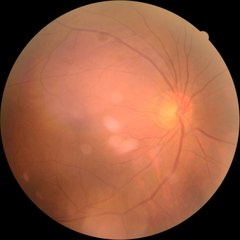
\includegraphics[width=1.62cm]{fundus.jpg}}; \end{scope}
  \draw[ink!80] (7.15,12.55) circle (0.78);
  \node[note] at (7.15,11.55) {input image $x$};
  \node[frz,minimum width=3.6cm,minimum height=2.2cm] (ienc) at (10.15,12.55) {};
  \node[btitle] at (10.15,13.35) {CLIP image encoder};
  \node[note] at (10.15,12.98) {ResNet-50 (frozen)};
  \node[trn,text width=3.0cm] (lora) at (10.15,12.1) {\textbf{LoRA} $r{=}16$, $\alpha{=}16$\\ all conv layers, 1.19\,M};
  \draw[arr] (7.95,12.55) -- (ienc.west);
  \foreach \i in {0,...,5} \fill[outln!55,draw=white] (12.55,12.0+0.19*\i) rectangle ++(0.3,0.19);
  \node[note,anchor=north,align=center,inner sep=1pt] at (12.85,11.92) {$z\in\mathbb{R}^{1024}$\\ $\ell_2$-normalised};
  \draw[arr] (ienc.east) -- (12.5,12.55);}

% similarity heat map S (B x 5) at the top right of panel (b)
\newcommand{\simmatrix}[1]{\simmatrixT{Similarity $S$}{#1}}
\newcommand{\simmatrixT}[2]{%
  \node[outb,minimum width=3.0cm,minimum height=2.7cm] (S) at (16.2,12.4) {};
  \node[btitle] at (16.2,13.45) {#1};
  \foreach \r/\row in {0/{100,55,25,8,3},1/{40,100,55,25,8},2/{8,40,100,55,25},3/{3,8,40,100,55}} {
    \foreach \v [count=\c from 0] in \row {\fill[outln!\v,draw=white] (15.25+0.38*\c,13.0-0.32*\r) rectangle ++(0.38,-0.32);}}
  \node[font=\scriptsize] at (16.2,11.35) {#2};
  \draw[arr] (12.9,12.55) -- (S.west);}

% ordinal grade axis at the bottom of panel (b)
\newcommand{\gradeaxis}[1]{%
  \node[blk,minimum width=11.4cm,minimum height=1.9cm] at (11.9,3.75) {};
  \node[anchor=west,font=\footnotesize\bfseries] at (6.35,4.45) {Ordinal grade axis};
  \node[anchor=east,cite] at (17.5,4.45) {#1};
  \draw[->,line width=1pt,ink!70] (6.8,3.65) -- (17.3,3.65);
  \foreach \g/\c/\n in {0/g0/No DR,1/g1/Mild,2/g2/Moderate,3/g3/Severe NPDR,4/g4/PDR} {
    \fill[\c] (7.6+2.2*\g,3.65) circle (0.12);
    \node[font=\scriptsize,below=2pt] at (7.6+2.2*\g,3.55) {\g\ $\cdot$ \n};}}

% (d) protocol strip: #1 = list of chip texts separated by |
\newcommand{\protocol}[1]{%
  \panel{0.2}{0.15}{25.8}{2.35}{(d)}{Experimental protocol}
  \def\px{0.4}
  \foreach \t [count=\i] in {#1} {\node[pchip,anchor=west,text width=3.9cm] at (0.35+4.24*\i-4.24,0.95) {\t};}}

% prediction and evaluation box at the bottom of panel (c); #1 = decision rule
\newcommand{\evalbox}[1]{%
  \node[outb,minimum width=7.3cm,minimum height=2.85cm] (ev) at (21.95,4.22) {};
  \node[btitle] at (21.95,5.3) {Prediction and evaluation (400 test images)};
  \node[font=\footnotesize] at (21.95,4.7) {#1};
  \foreach \m [count=\i from 0] in {\textbf{QWK} $\uparrow$,MAE $\downarrow$,Macro-F1 $\uparrow$,AUC $\uparrow$,Acc. $\uparrow$} \node[chip,minimum width=1.25cm] at (19.15+1.4*\i,3.95) {\m};
  \foreach \m [count=\i from 0] in {LOS $\uparrow$,ODC $\uparrow$,ECE $\downarrow$,NLL $\downarrow$,Brier $\downarrow$} \node[chip,minimum width=1.25cm] at (19.15+1.4*\i,3.35) {\m};
  \node[note] at (21.95,3.02) {QWK primary; errors should fall with distance from the diagonal};}

% ---------------------------------------------------------------------------
% Protocol figure (one per model): four numbered steps of a run, then what is compared.
%   \protocolfig{train lines}{size line}{baseline chips}{ablation chips}
% chips are written with \bchip{..} (baselines) and \achip{..} (ablations)
\newcommand{\bchip}[1]{{\setlength{\fboxsep}{2.2pt}\fcolorbox{outln!60}{outbg}{\strut #1}}\hspace{3pt}\allowbreak}
\newcommand{\achip}[1]{{\setlength{\fboxsep}{2.2pt}\fcolorbox{trnln!70}{trnbg}{\strut #1}}\hspace{3pt}\allowbreak}
\tikzset{
  pstep/.style={rounded corners=4pt,line width=0.7pt,minimum width=3.85cm,minimum height=3.3cm,anchor=north west},
  stepnum/.style={circle,fill=#1,text=white,font=\footnotesize\bfseries,inner sep=1.3pt,minimum size=5mm},
  steptext/.style={anchor=north west,text width=3.55cm,align=left,font=\footnotesize,inner sep=0pt},
  regchip/.style={rounded corners=2pt,draw=frzln,fill=frzbg,font=\scriptsize\bfseries,minimum width=7.2mm,minimum height=5mm,inner sep=0pt},
}
\newcommand{\protocolfig}[4]{%
  % step boxes
  \node[pstep,draw=frzln,fill=frzbg!45] (p1) at (0,0) {};
  \node[pstep,draw=trnln,fill=trnbg!55] (p2) at (4.3,0) {};
  \node[pstep,draw=statln,fill=statbg!60] (p3) at (8.6,0) {};
  \node[pstep,draw=outln,fill=outbg!70] (p4) at (12.9,0) {};
  \draw[arr,line width=1.1pt] (p1.east) -- (p2.west);
  \draw[arr,line width=1.1pt] (p2.east) -- (p3.west);
  \draw[arr,line width=1.1pt] (p3.east) -- (p4.west);
  \node[stepnum=frzln,anchor=west] at (0.2,-0.45) {1};  \node[anchor=west,font=\footnotesize\bfseries] at (0.8,-0.45) {Regimes and seeds};
  \node[stepnum=trnln,anchor=west] at (4.5,-0.45) {2};  \node[anchor=west,font=\footnotesize\bfseries] at (5.1,-0.45) {Train on the support};
  \node[stepnum=statln,anchor=west] at (8.8,-0.45) {3}; \node[anchor=west,font=\footnotesize\bfseries] at (9.4,-0.45) {Select on the query};
  \node[stepnum=outln,anchor=west] at (13.1,-0.45) {4}; \node[anchor=west,font=\footnotesize\bfseries] at (13.7,-0.45) {Test once};
  % step 1: the eight regimes as chips
  \foreach \r [count=\i from 0] in {ZS,1,2,4,8,16,32,Full}
    \node[regchip] at ({0.6+0.88*mod(\i,4)},{-1.35-0.68*int(\i/4)}) {\r};
  \node[steptext,font=\scriptsize] at (0.18,-2.35) {$k$ = images per grade\\ $\times$ 3 seeds $=$ \textbf{24 runs}};
  % steps 2-4
  \node[steptext] at (4.48,-0.95) {#1\\[3pt] {\color{sub}#2}};
  \node[steptext] at (8.78,-0.95) {validate after every epoch\\ QWK on the query set\\ early stop: patience 20\\ keep \texttt{best} and \texttt{last}};
  \node[steptext] at (13.08,-0.95) {best checkpoint on the\\ 400 test images (100 patients)\\[3pt] \textbf{QWK} (primary), MAE, F1, AUC, ODC, ECE, NLL, Brier};
  % comparison row
  \node[rounded corners=4pt,draw=outln!70,fill=white,line width=0.6pt,anchor=north west,minimum width=8.3cm,minimum height=2.45cm] (cb) at (0,-3.75) {};
  \node[anchor=north west,font=\footnotesize\bfseries] at (0.2,-3.9) {Compared against};
  \node[anchor=north west,text width=7.9cm,align=left,font=\footnotesize] at (0.2,-4.4) {#3};
  \node[rounded corners=4pt,draw=trnln!80,fill=white,line width=0.6pt,anchor=north west,minimum width=8.3cm,minimum height=2.45cm] (ab) at (8.45,-3.75) {};
  \node[anchor=north west,font=\footnotesize\bfseries] at (8.65,-3.9) {Ablations \textmd{\color{sub}(one change each, same 24-run protocol)}};
  \node[anchor=north west,text width=7.9cm,align=left,font=\footnotesize] at (8.65,-4.4) {#4};
}
